% METODOLOGIA------------------------------------------------------------------

\chapter{METODOLOGIA}
\label{chap:metodologia}
Nesta seção será abordada a forma de desenvolvimento de um algoritmo focado na análise de \textit{copy number variation} a partir de algoritmos especializados na detecção de \textit{change point}, além de ser apresentado os dados fonte, as tecnologias e o recurso de validação a ser utilizados no método proposto. 

\section{MÉTODO PROPOSTO} 

O método proposto é desenvolver um algoritmo de segmentação de dados do exoma, capaz de utilizar mais de um método de detecção de ponto de mudança. A estrutura do algoritmo deverá ser capaz de executar a leitura de dados de exoma, disponibilização de formas de escolha de métodos de segmentação e de retornar os dados segmentados apresentando informações críticas como a existência de alguma variação no número de cópias.

O projeto deverá ser produzido na Linguagem R, para facilitar a utilização e integração de projetos existentes que detectam pontos de mudanças. Ele se baseará em fonte como o DNAcopy \cite{Olshen2004} para o desenvolvimento e leitura dos dados.

\section{TECNOLOGIAS UTILIZADAS}

Nesta seção serão descritos as tecnologias utilizadas para o desenvolvimento do projeto, apresentando uma breve contextualização e definindo conceitos essenciais para o entendimento do ambiente de criação da pesquisa.

\subsection{R}

O R \cite{Core2019} é uma linguagem e um ambiente focado em computação estatística e gráficos, contendo um módulo complementar incluso ao seu ambiente com vários pacotes de procedimentos estatístico, apresentação de dados gráficos e outros disponibilizados para o uso nos mais diversos contextos \cite{website:Hornik2018}.

O R permite a criação de \textit{scripts} de execução, que são responsáveis por variados tipos de comandos, desde contas matemáticas simples como uma soma, até a execução de algoritmos complexos e ou exibição de gráficos sobre determinados dados. A plataforma permite o agrupamento de variados \textit{scripts} em subdiretórios (pasta de trabalho) para obter uma maior organização a nível de código, possibilitar os testes, a documentação e a distribuição dos códigos criados, o conjunto de todos os arquivos referentes a essa estrutura é denominada como pacote \cite{website:Hornik2018}.

\subsubsection{PACOTES R}

O pacote R é uma forma de agrupar um código em um padrão de projeto para que seja mais fácil a distribuição e a utilização por terceiros, a disponibilização da maioria do pacotes R é contida na plataforma CRAN \cite{website:Hornik2018}.

\begin{quadro}[hbp]
\centering
\caption{Pacotes R de algoritmos de detecção de pontos de mudança \label{qua:ferramtas-cpd}}
    \begin{adjustbox}{max width=\textwidth}
    \begin{tabular}{ | c | c | p{5cm} | p{5cm} | } \hline
        \textbf{Nome}     & \textbf{Versão}      & \textbf{Algoritmo}     & \textbf{Referência} \\ \hline
        bcp & 4.0.3 &  & \cite{Emerson2007} \\ \hline
        breakfast & 1.1.1 &  & \cite{Fryzlewicz2017} \\ \hline
        changepoint & 2.2.2 &  & \cite{Eckley2016} \\ \hline
        SpecDetec & 1.0.0 &  & \cite{Uzai2018} \\ \hline
    \end{tabular}
    \end{adjustbox}
\end{quadro}

\subsubsection{CRAN}

O \textit{Comprehensive R Archive Network} (CRAN) é uma plataforma para o arquivamento de pacotes R, para facilitar o acesso a versões e informações críticas de um pacote, como a documentação e as instruções de instalação. A partir dele é possível a obtenção de binários pré-construídos para vários sistemas operacionais (Linux, Mac OS Classic, macOS e MS Windows), arquivos zipados e outros. Os pacotes distribuídos pelo CRAN está disposto a comunidade para utilização, devido a sua natureza \textit{open source} \cite{website:Hornik2018}.

\subsection{GitHub}

O GitHub \cite{GitHub2019} é uma plataforma de hospedagem de código-fonte versionado pelo Git\footnote{Sistema de controle de versões de projetos, capaz de registrar o histórico de edições}, ele dispõe de funcionalidades do Git em interface ráfica e acrescenta recursos necessários para a colaboração em repositórios públicos e privados, além de oferecer ferramentas e extensões para o controle de projetos. O GitHub amplamente utilizada e já chegou a registrar três milhões de projetos mantidos por mais de um milhão de desenvolvedores registrados \cite{Thung2013}.

\section{DESENVOLVIMENTO}

\subsection{Visão Geral}

A construção do projeto proposto será implantada na linguagem R, seguindo os padrões sugeridos ao criar um pacote para que a distribuição dele possa ser feita pelo CRAN. O código-fonte e documentação produzida serão armazenadas de forma \textit{open source} nas plataformas do GitHub e CRAN, facilitando o controle de versão e a contribuições futuras ao projeto.

Para a criação do projeto será usado como base algumas das ferramentas especificas para busca de CNVs, se baseando na estrutura delas para formulação de um ambiente especializado em leituras de dados sequenciado do exoma. Uma das principais fonte de dados na qual o projeto se baseará será o DNAcopy, retirando ideias e conceitos semelhantes.

A segmentação dos dados será dada pela integração de pacotes de detecção de ponto de mudanças contidos no CRAN, adaptando-os se necessário para que eles possam identificar as variações do exoma.

\subsubsection{Fluxo de Funcionamento}

O modelo de processo de funcionamento descrito na \autoref{fig:metodologia-tcc}, terá 2 etapas de responsabilidade do usuário, sendo elas entrada de dados, configurações iniciais. A partir da inserção das informações pedidas ao usuário, o algoritmo será capaz de realizar o processamento das informações inseridas em 4 etapas de execução, preparação dos dados, aplicação da segmentação, identificação dos pontos de mudança e a organização dos resultados e informações inseridas.

\begin{figure}[!htb]
    \centering
    \caption{Representação gráfica do processo de detecção de pontos de mudança com múltiplos algoritmos de segmentação}
    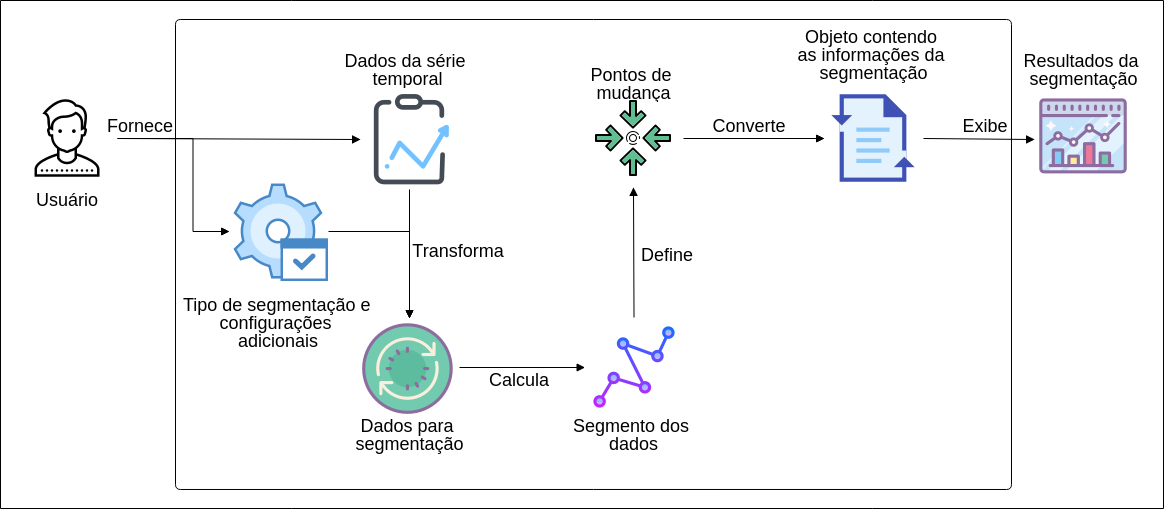
\includegraphics[width=1\textwidth]{./dados/figuras/metodologia-tcc}
    \fonte{Autoria Própria}
    \label{fig:metodologia-tcc}
\end{figure}

O procedimento de escolha de algoritmos é representado na (Figura 6), de forma a exemplificar o modelo de seleção a ser usado como base no desenvolvimento do projeto. Os métodos de segmentação de entrada serão escolhidos por meio de parâmetros na função de segmentação, assim podendo ser identificado qual método escolhido e quais atributos adicionais serão inseridos referente ao modelo de segmentação selecionado. 

A partir da segmentação a saída dos resultados serão padronizadas contendo os dados de entrada, os resultados dos cálculos e informações referentes a chamada da função, descrevendo quais os parâmetros utilizados no cálculo dos pontos de mudança. Portanto, com o objeto retornado será possível plotar gráficos de acordo com o desejo do usuário, ao usar a função de plotar da linguagem R.

\section{BASE DE DADOS} 
\label{sec:baseDeDados} 

Com o objetivo de testar o desempenho e funcionamento do algoritmo criado, os dados dados do Coriell \cite{Snijders2001} será utilizado, utilizando as linhas celulares disponibilizadas pelo projeto. Esses dados são utilizados em vários projetos similares, como o DNAcopy \cite{Olshen2004} e \cite{Girimurugan2018}. Entretanto, caso haja a necessidade, será retirado informações de outros sequenciamentos do Banco de Exoma.

A base de dados disponibilizadas como Coriell possui informações relevantes sobre a linha celular, como o clone que as informações foram tiradas, o cromossomo de referência, a sua variação e assim por diante. A estrutura presente nas informações disponibilizadas do coriell é semelhante a \autoref{tab:tabela-2-dados}, onde são apresentadas os cinco primeiros elementos referente a linha celular do GM05296 e GM13330, dispostas pelo Coriell \cite{Snijders2001}. 

% ######## init table ########
\begin{table}[h]
 \centering
% distancia entre a linha e o texto
 {\renewcommand\arraystretch{1.25}
 \caption{Cinco primeiros dados do Coriell correspondentes a amostra GM05296 e GM13330 contidos na base do DNAcopy}
 \label{tab:tabela-2-dados}
 \begin{tabular}{ l l l l l }
  \cline{1-1}\cline{2-2}\cline{3-3}\cline{4-4}\cline{5-5}  
    \multicolumn{1}{c}{Clone \centering } &
    \multicolumn{1}{c}{Chromosome \centering } &
    \multicolumn{1}{c}{Position \centering } &
    \multicolumn{1}{c}{Coriell.05296 \centering } &
    \multicolumn{1}{c}{Coriell.13330 \centering }
  \\  
  \cline{1-1}\cline{2-2}\cline{3-3}\cline{4-4}\cline{5-5}  
    \multicolumn{1}{c}{GS1-232B23 \centering } &
    \multicolumn{1}{c}{1 \centering } &
    \multicolumn{1}{c}{0 \centering } &
    \multicolumn{1}{c}{NA \centering } &
    \multicolumn{1}{c}{0.207470 \centering }
  \\  
  \cline{1-1}\cline{2-2}\cline{3-3}\cline{4-4}\cline{5-5}  
    \multicolumn{1}{c}{RP11-82d16 \centering } &
    \multicolumn{1}{c}{1 \centering } &
    \multicolumn{1}{c}{468 \centering } &
    \multicolumn{1}{c}{0.008824 \centering } &
    \multicolumn{1}{c}{0.063076 \centering }
  \\  
  \cline{1-1}\cline{2-2}\cline{3-3}\cline{4-4}\cline{5-5}  
    \multicolumn{1}{c}{RP11-62m23 \centering } &
    \multicolumn{1}{c}{1 \centering } &
    \multicolumn{1}{c}{2241 \centering } &
    \multicolumn{1}{c}{-0.000890 \centering } &
    \multicolumn{1}{c}{0.123881 \centering }
  \\  
  \cline{1-1}\cline{2-2}\cline{3-3}\cline{4-4}\cline{5-5}  
    \multicolumn{1}{c}{RP11-60j11 \centering } &
    \multicolumn{1}{c}{1 \centering } &
    \multicolumn{1}{c}{4504 \centering } &
    \multicolumn{1}{c}{0.075875 \centering } &
    \multicolumn{1}{c}{0.154343 \centering }
  \\  
  \cline{1-1}\cline{2-2}\cline{3-3}\cline{4-4}\cline{5-5}  
    \multicolumn{1}{c}{RP11-111O05 \centering } &
    \multicolumn{1}{c}{1 \centering } &
    \multicolumn{1}{c}{5440 \centering } &
    \multicolumn{1}{c}{0.017303 \centering } &
    \multicolumn{1}{c}{-0.043890 \centering }
  \\  
  \hline

 \end{tabular} }
 \fonte{Autoria Própria}
\end{table}

\section{VALIDAÇÃO} 

O método proposto necessitará ser validado para que haja uma garantia de que os pontos de mudanças sejam conservados no mesmo local, assim obtendo uma maior veracidade na confiança do trabalho desenvolvido. Portanto, para garantir efetividade do algoritmo será utilizado a Matriz de Confusão aplicada aos dados descritos na \autoref{sec:baseDeDados} para obter uma análise do desempenho do algoritmo.